\section{Meltdown}
In this section we will explain how Meltdown attack works and how we managed to
test it on our machines. This paper has the target of explaining how Meltdown works in a more "human readable" manner, and so we will provide pseudocode along with
assembly code for reference.

\subsection{Terminology}
Meltdown resarchers have used their own terminology which helps the reader to better understand the main concepts.

Transient instructions are those instructions that are executed out-of-order, meaning those instructions that, in a program logic, should be executed
after another instruction but, because of the micro-architecture of che processor, are executed at the same time.

Transient instruction sequence is a sequence of transient instructions.

\subsection{How it works}
Meltdown attacks consists of 3 main steps:

\begin{enumerate}[label={Step \arabic*:}]
    \item Load content of (inaccessible) memory location on a register
    \item Allocate "Probe Array" on main memory
    \item Use the previosly loaded data to transimt secret on a legitimate instruction execution
    \item Store leaked secret on main memory leveraging Flush+Reload and previosly allocated Probe Array
\end{enumerate}


\subsubsection{Step 1: Fetch privileged data}
Meltdown's main objective is to get privileged data from main memory which is otherwise inaccessible, and to do so
the attack starts with simple access to an unauthorized memory location.
In our example we will refer to such address as the "0xABC0" memory address, which our code is not autorized to access to,
which points to the first byte of an array containing our secret ("Meltdown").
So our secret is stored from "0xABC0" (`m', first letter) to "0xABC7" (`n', last letter).

\begin{verbatim}
...
   secret = readAddress(0xABC0);
...
\end{verbatim}
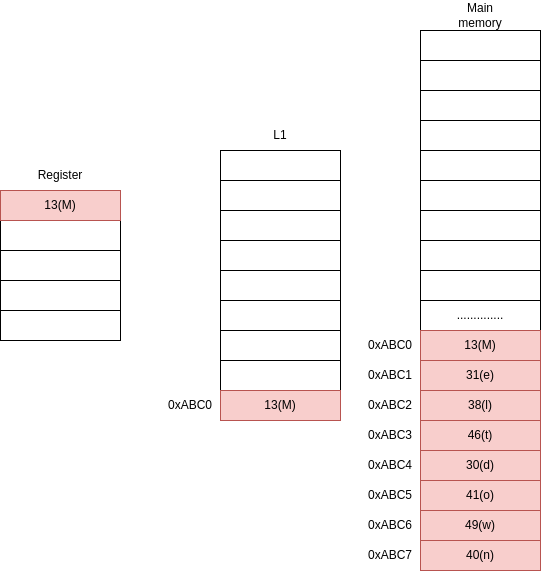
\includegraphics[scale=0.25]{img/meltdown-step-one.png}


\subsubsection{Step 2: Allocate Probe Array}
In our example, we allocate a so called Probe Array which holds an array of "acceptable" values for our secret.
\begin{verbatim}
...
    secret = readAddress(0xABC0);
    probe_array=no_cache_array("A", "B", "C", ... 
                , "Z", "a", ... "z");

...
\end{verbatim}
For the sake of simplicity, no\_cache\_array is a function that allocates an array without caching.
For example, accessing to probe\_array[2] will result, at current micro-architectural state, in a "cache miss".
This is a fundamental step for out-of-order exploitation.
On the flush+reload step, what we want is that none of the pages holding these data is loaded but the one which store the value
"M" since it is the first char of the secret value.

\subsubsection{Step 3: Transmit secret}
Now we have a register containing the value of the accessed secret and an array that contains all possible values that secret may be equal to,
all is left to do is to legitimately get that value in order to store it on the main memory without the Reservation Station deleting its result
after realizing that we should have not accessed that location genearting an architectural exception (also called "trap").
\begin{verbatim}
...
    secret = readAddress(0xABC0);
    probe_array=no_cache_array("A", "B", "C", ... 
                , "Z", "a", ... "z");
    probe_array(secret);
...
\end{verbatim}

What we oversimplified on line 3 is what loads the desired page on our core cache. On a micro-architectural level, accessing the secret-th value of probe\_array
will first result on a "cache miss" and then the processor loads the value from main memory into the cache.
Note that the pseudocode we provide dosen't really make sense on a more realistic lens, since we are assuming that the address "0xABC0" is storing the exact
offset in which the value is stored on our probe\_array. In a more realistic example we should first load the value on a register, e.g. RAX,
and then translate that value in something that can be used to retrive a specific page from the memory which,
like hasing functions, is equal to a well-known value. Also, an important note here is that each page
of probe\_array contains exactly and only a single value, being "A" for the first page, "B" for the second, and so on until "z".

\subsubsection{Step 4: Flush+Reload to store the value}
At this point all that's left to do is to store the secret value in a manner that Reservation Station will not delete its result.
\begin{verbatim}
...
    secret = readAddress(0xABC0);
    probe_array=no_cache_array("A", "B", "C", ... 
                , "Z", "a", ... "z");
    probe_array(secret);
    for(i = 0; i < 52; i++){
        cycle_count_set(0);
        probe_array(i);
        if(cycle_count_get < 100) p = probe_array(i);
        clflush(probe_array(i))
    }
...
\end{verbatim}

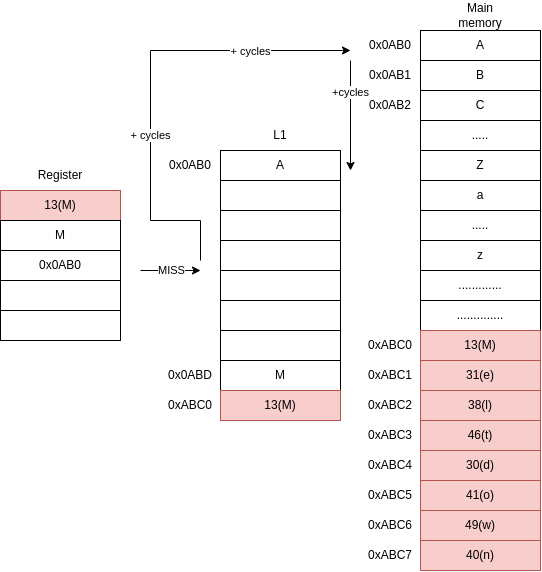
\includegraphics[scale=0.25]{img/meltdown-step-two.png}
\newline
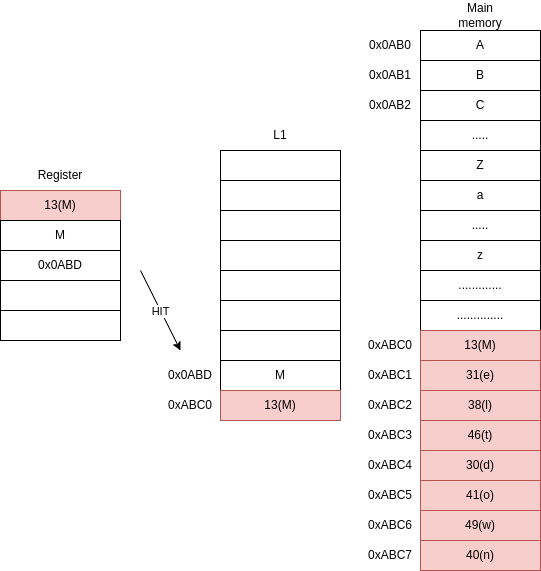
\includegraphics[scale=0.25]{img/meltdown-step-four.png}
\newline
In our example, we iterate every page relevant to our probe\_array in order to leverage Flush+Reload technique previosly discussed.
We iterate all 52 pages of the probe\_array and measure how cycles does it take to load the value: in our assumptions, if the cycle count
is lesser than 100, then the page was already on cache, which means that line 3 was the last and the only who could have done that.
we now procede to save the value on a register which will not be ereased by the Reservation Station since Line 7 is not doing anything wrong
from the point of view of the Reservation Station. On Line 8 we flush the cache line so to leave pages of probe\_array unloaded until we read the next privileged address.

\subsection{More realistic example}

